\section{Omówienie działania głębokich sieci neuronowych}
\subsection{Wprowadzenie do sieci neuronowych}

Podstawowymi elementami strukturalnymi, z których buduje się sztuczne sieci 
neuronowe są neurony. Każdy neuron posiada wejścia, na które podawane są 
sygnały mnożone przez odpowiednie wagi, sumowane, a następnie po przejściu przez 
funkcje aktywacji kierowane na wyjście neuronu. 


\begin{figure}[H]
	\centering
	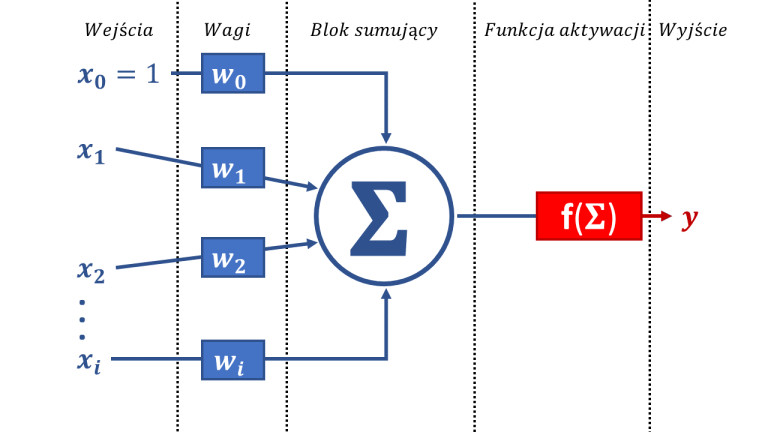
\includegraphics[width=12cm]{pages/teoria/zdjecia/sztucznyNeuron.jpg}
	\caption{Schemat pojedynczego neuronu \cite{sztucznyNeuron}}
	\label{rys:ogolnyRozwiazania}
\end{figure}


Wyjście powyższego neuronu możemy opisać wzorem:

\begin{equation}
	y = f( \sum_{i = 0}^{N}w_i x_i) = f(W^T x)
	\label{eq:rownanieNeuronu}
\end{equation}
Gdzie: $x=[1, x_1, x_2, ..., x_N]$ - to wektor sygnałów wejściowych (1 na początku wektora odpowiada
za przesunięcie), $W = [w_0, w_1, w_2, ..., w_N]$ - jest wektorem wag ($w_0$ to wartość progowa aktywacji),
$f(x)$ to wybrana funkcja aktywacji

\textbf{Najczęściej stosowane funkcje aktywacji:}

\begin{equation}
	f(x) = \frac{1}{1 + e^-x\beta} 
	\label{eq:signum}
\end{equation}

\begin{equation}
	f(x) = \frac{e^x - e^-x}{e^x + e^-x}
	\label{eq:tangensHiperboliczny}
\end{equation}

\begin{equation}
	f(x) = \begin{cases}
		1 & gdy x \> 0 \\
		0 & gdy x <  0
	\end{cases}
	\label{eq:skokuJednostkowego}
\end{equation}


\textbf{Wielowarstwowe sieci neuronowe}

W praktycznym zastosowaniu sieć zbudowana z jednej warstwy neuronów nie pozwoli nam na osiągnięcie satysfakcjonujących wyników.
Możemy określić dwa typy sieci pod względem ilości warstw: 
\begin{itemize}
	\item Uczenie maszynowe - zazwyczaj są zbudowane z trzech warstw (ukryta-ukryta-wyjściowa) 
	\item Głębokie uczenie - posiada dużo więcej warstw neuronów, w skomplikowanych sieciach nawet kilkaset
\end{itemize}

Relacje pomiędzy nimi przedstawia poniższy schemat
\begin{figure}[H]
	\centering
	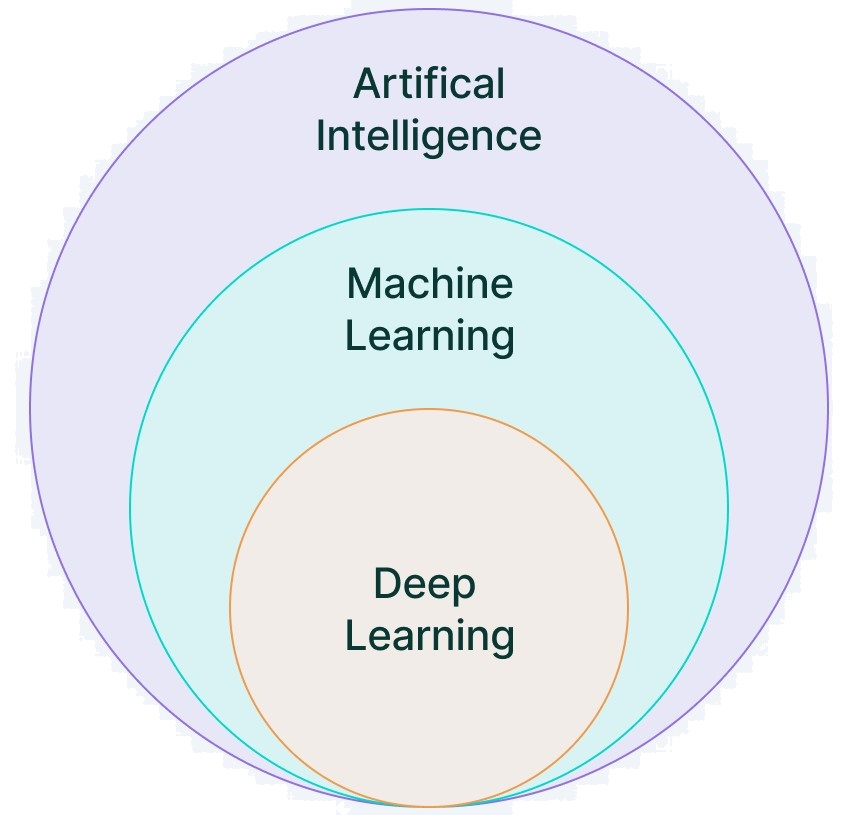
\includegraphics[width=10cm]{pages/teoria/zdjecia/schematAI.jpg}
	\caption{Relacja pomiędzy typami sieci neuronowych \cite{schematAISite}}
	\label{rys:schematAI}
\end{figure}


\subsection{Głębokie sieci neuronowe}


\subsection{Algorytmy detekcji obiektów na zdjęciach}

